% Fig. 1  System architecture (double column, drawn at 7.1 in).
% Provenance: backend/insightflow/orchestrator.py module docstring and step 12b (commit b11793b);
% evaluation harness evaluation/v3/run_eval.py calls Orchestrator().ask(q) directly.
\documentclass[border=2pt]{standalone}
% Shared settings for all InsightFlow AI figures (Times, grayscale, sized for IEEE print).
\usepackage[T1]{fontenc}
\usepackage{mathptmx}
\usepackage{tikz}
\usetikzlibrary{positioning,arrows.meta,calc,fit,patterns,shapes.geometric}
\tikzset{
  >={Stealth[length=4pt,width=3.5pt]},
  stage/.style={draw,rounded corners=1.5pt,fill=gray!8,align=center,inner sep=2.5pt,font=\fontsize{7.5}{8.6}\selectfont},
  ext/.style={draw,dashed,rounded corners=1.5pt,align=center,inner sep=2.5pt,font=\fontsize{7.5}{8.6}\selectfont},
  note/.style={align=left,font=\fontsize{7}{8}\selectfont},
  flow/.style={->,thick},
  dflow/.style={->,dashed},
  every node/.append style={execute at begin node={\hyphenpenalty=10000\exhyphenpenalty=10000}},
}

\begin{document}
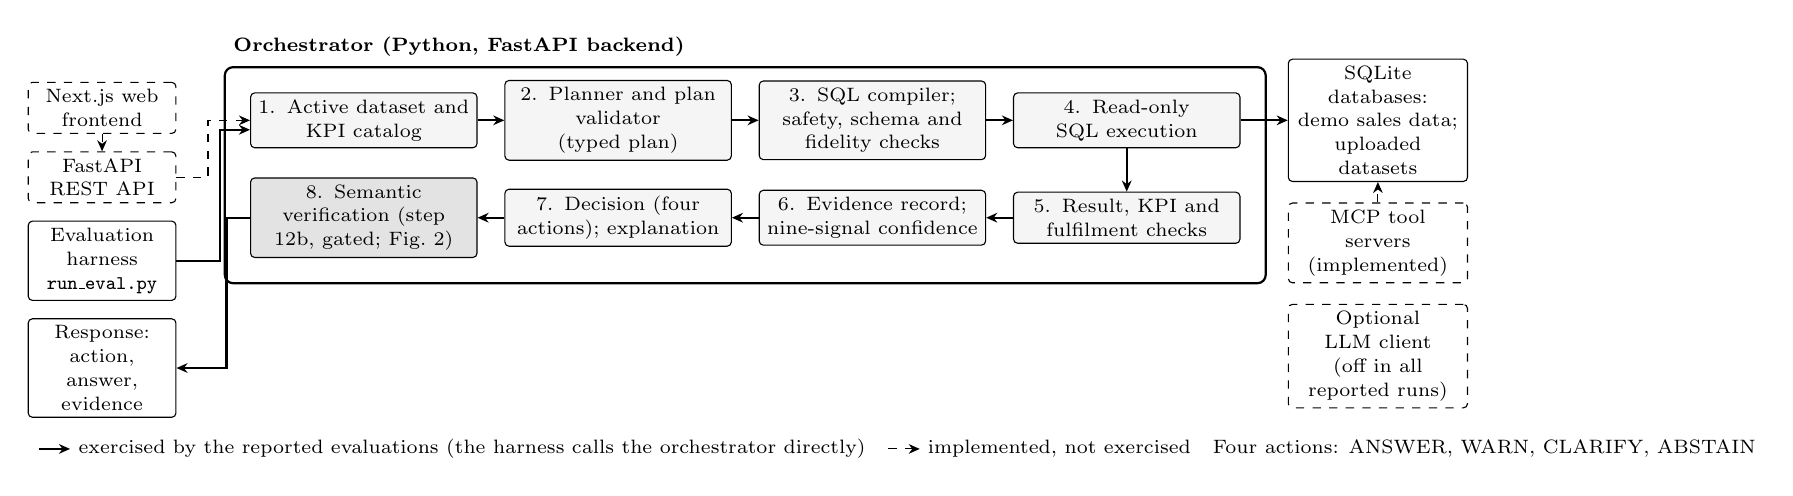
\begin{tikzpicture}[node distance=3.2mm and 3.4mm]
  \def\w{27mm}
  % orchestrator stages, row 1 (left to right)
  \node[stage,text width=\w] (s1) {1. Active dataset and\\KPI catalog};
  \node[stage,text width=\w,right=of s1] (s2) {2. Planner and plan\\validator (typed plan)};
  \node[stage,text width=\w,right=of s2] (s3) {3. SQL compiler;\\safety, schema and\\fidelity checks};
  \node[stage,text width=\w,right=of s3] (s4) {4. Read-only\\SQL execution};
  % row 2 (right to left)
  \node[stage,text width=\w,below=5.5mm of s4] (s5) {5. Result, KPI and\\fulfilment checks};
  \node[stage,text width=\w,left=of s5] (s6) {6. Evidence record;\\nine-signal confidence};
  \node[stage,text width=\w,left=of s6] (s7) {7. Decision (four\\actions); explanation};
  \node[stage,text width=\w,left=of s7,fill=gray!22] (s8) {8. Semantic\\verification (step\\12b, gated; Fig.~2)};
  \draw[flow] (s1) -- (s2); \draw[flow] (s2) -- (s3); \draw[flow] (s3) -- (s4);
  \draw[flow] (s4) -- (s5); \draw[flow] (s5) -- (s6); \draw[flow] (s6) -- (s7); \draw[flow] (s7) -- (s8);
  \node[draw,thick,rounded corners=3pt,inner sep=3.2mm,fit=(s1)(s4)(s5)(s8)] (orch) {};
  \node[anchor=south west,font=\fontsize{7.5}{8.6}\selectfont\bfseries] at (orch.north west) {Orchestrator (Python, FastAPI backend)};
  % inputs on the left
  \node[ext,text width=17mm,left=6mm of orch.north west,anchor=north east,yshift=-2mm] (ui) {Next.js web\\frontend};
  \node[ext,text width=17mm,below=2.2mm of ui] (api) {FastAPI\\REST API};
  \node[stage,text width=17mm,below=2.2mm of api,fill=white] (harness) {Evaluation harness\\\texttt{run\_eval.py}};
  \draw[dflow] (ui) -- (api);
  \draw[dflow] (api.east) -- ++(4mm,0) |- (s1.west);
  \draw[flow] (harness.east) -- ++(5.5mm,0) |- ([yshift=-1.2mm]s1.west);
  \node[stage,text width=17mm,below=2.2mm of harness,fill=white] (resp) {Response: action,\\answer, evidence};
  \draw[flow] (s8.west) -- ++(-3mm,0) |- (resp.east);
  % data and tools on the right
  \node[stage,text width=21mm,right=6mm of s4,fill=white] (db) {SQLite databases:\\demo sales data;\\uploaded datasets};
  \draw[flow] (s4) -- (db);
  \node[ext,text width=21mm,below=2.6mm of db] (mcp) {MCP tool servers\\(implemented)};
  \draw[dflow] (mcp) -- (db);
  \node[ext,text width=21mm,below=2.6mm of mcp] (llm) {Optional LLM client\\(off in all\\reported runs)};
  % legend
  \node[note,anchor=north west] at ([yshift=-1.5mm]resp.south west) {%
    \tikz[baseline=-0.6ex]\draw[thick,->](0,0)--(4mm,0); exercised by the reported evaluations (the harness calls the orchestrator directly)\quad
    \tikz[baseline=-0.6ex]\draw[dashed,->](0,0)--(4mm,0); implemented, not exercised\quad
    Four actions: ANSWER, WARN, CLARIFY, ABSTAIN};
\end{tikzpicture}
\end{document}
